\subsection{iSAM}
\subsubsection{Getting to SLAM update step}
Before we can compute a good estimate, we need a simple model of how the robot moves and how sensors observe the world. We use a motion model for state evolution and a measurement model for sensor readings. States are $x_i$ (robot poses), controls are $u_i$, and measurements $z_k$ (landmarks). We stack all unknowns into $\theta$ (poses and landmarks).
\\ \\
Motion (process) model:
$$
    \begin{aligned}
        x_i = f_{i}(x_{i-1}, u_i) + w_i \\ 
        w_i \sim N(0, Q_i) \qquad
    \end{aligned}
$$
Given the previous state $x_{i-1}$ and control $u_i$, the next state $x_i$ comes from a model $f$ plus uncertainty noise in the model itself $w_i$. This uncertainty captures things like currents, slip, and actuator errors. $f_i$ can be a discrete time dynamics update or use plain odometry. Assuming Gaussian $w_i$ is a handy start so \gls{MAP} becomes least squares. Later we can switch uncertainty model to robust or heavy tailed noise if needed.
\\ \\
Measurement model:
$$
    \begin{aligned}
        z_k = h_{k}(x_{i_k}, l_{j_k}) + v_k \\ 
        v_k \sim N(0, R_k) \qquad
    \end{aligned}
$$
Each measurement $z_k$ depends on state $x_{i_k}$ and landmarks $l_{j_k}$ transformed using measurement transform function $h_{k}(\cdot)$, this allows state estimate to become estimated measurement position. In addition this measurement has noise $v_k$ witch we model ad Gaussian noise for simplifications later on when calculating.
\\ \\
Prior:
$$
    \begin{aligned}
        x_0 \sim N(\mu_{0}, \Sigma_{0})
    \end{aligned}
$$
A prior anchors the graph (otherwise the problem is underdetermined up to a global transform). It can encode GPS at the start, a known dock pose, or simply a weak ``zero'' prior to fix gauge.
\\ \\
We want our predictions to match measurements. In a perfect world, every residual (prediction minus measurement) would be zero. In reality we have model errors and sensor noise, so residuals are nonzero. Estimation is about choosing the state update that makes all residuals as small and as statistically consistent as possible.
\\ \\
This is where MAP algorithm comes in. MAP (Maximum A Posteriori) is the principled way to fuse everything we know. A prior on the state, the motion model, and all measurements. It combines them through probability, weighting each residual by its uncertainty. With Gaussian noise, the negative log posterior becomes a sum of squared (weighted) residuals. That gives us a single objective to minimize, where more reliable terms (small covariance) count more. This is better than ad hoc weighting and naturally handles many sensors.
\\ \\
Our motion and measurement functions are nonlinear (angles, rotations, ranges). Minimizing the nonlinear MAP cost directly is hard. Linearization lets us solve it iteratively. At the current estimate we approximate the nonlinear functions by their first order Taylor expansion, solve a linear least squares problem for a small increment, update the estimate, and repeat. This is all shown in the iSAM paper \cite{iSAM_paper} where linearized forms of our system becomes:
\begin{equation}
    \begin{aligned}
        f_{i}(x_{i-1}, u_i) - x_i \approx (F_{i}^{i-1}\Delta x_{i-1} - \Delta x_{i}) - a_i \\
        \left.F_{i}^{i-1} := \frac{\partial f_{i}(x_{i-1}, u_i)}{\partial x_{i-1}}\right|_{x_{i-1}^{0}} \\ 
        a_i = x_{i-1}^{0} - f_{i}(x_{i-1}^{0}, u_i)
    \end{aligned}
    \label{eq:optimizer-iSAM-linearized-odometry}
\end{equation}
\begin{equation}
    \begin{aligned}
        h_{k}(x_{i-1}, u_i) - z_k \approx (H_{k}^{i_k}\Delta x_{i_k} - J_{k}^{j_k} \Delta l_{j_k}) - c_k \\
        \left.H_{k}^{i_k} := \frac{\partial h_{k}(x_{i_k}, l_{j_k})}{\partial x_{i_k}}\right|_{(x_{i_k}^{0}, l_{j_k}^{0})} \\ 
        \left.J_{k}^{j_k} := \frac{\partial h_{k}(x_{i_k}, l_{j_k})}{\partial l_{j_k}}\right|_{(x_{i_k}^{0}, l_{j_k}^{0})} \\ 
        c_k = z_{k} - h_{k}(x_{i_k}^{0}, l_{j_k}^{0})
    \end{aligned}
    \label{eq:optimizer-iSAM-linearized-measurement}
\end{equation}
\\ \\
Now we can plug the linearized forms of the odometry (\ref{eq:optimizer-iSAM-linearized-odometry}) and measurement models (\ref{eq:optimizer-iSAM-linearized-measurement}) into a single least squares estimator. After linearization, the problem becomes ``find the small state change $\Delta\theta$ that best reduces all residuals at once''. To keep the notation uniform, we treat the current pose increment like any other variable (that's why $G_{i}^{i}=-I$ appears). Next, we whiten each term, ie pre multiply by the square root of the inverse covariance so every residual has unit variance. For scalars, this is just dividing by the measurement standard deviation. Whitening turns all the weighted (Mahalanobis) errors into plain Euclidean errors, so we can drop the covariance symbols and stack everything into one big, sparse least squares system.
\begin{equation}
    \begin{aligned}
        \Delta\theta^{*} = 
        \arg\min_{\Delta\theta}\left\{ 
            \sum_{i=1}^{M}{\|F_{i}^{i-1}\Delta x_{i-1} + G_{i}^{i}\Delta x_{i} - a_i\|_{\Lambda_i}^{2}} +
            \sum_{k=1}^{K}{\|H_{k}^{i_k}\Delta x_{i_k} + J_{k}^{j_k} \Delta l_{j_k}) - c_k\|_{\Gamma_k}^{2}}
            \right\}
    \end{aligned}
    \label{eq:optimizer-iSAM-delta-theta-star-mahalanobis-form}
\end{equation}
\begin{figure}[H]
    \centering
    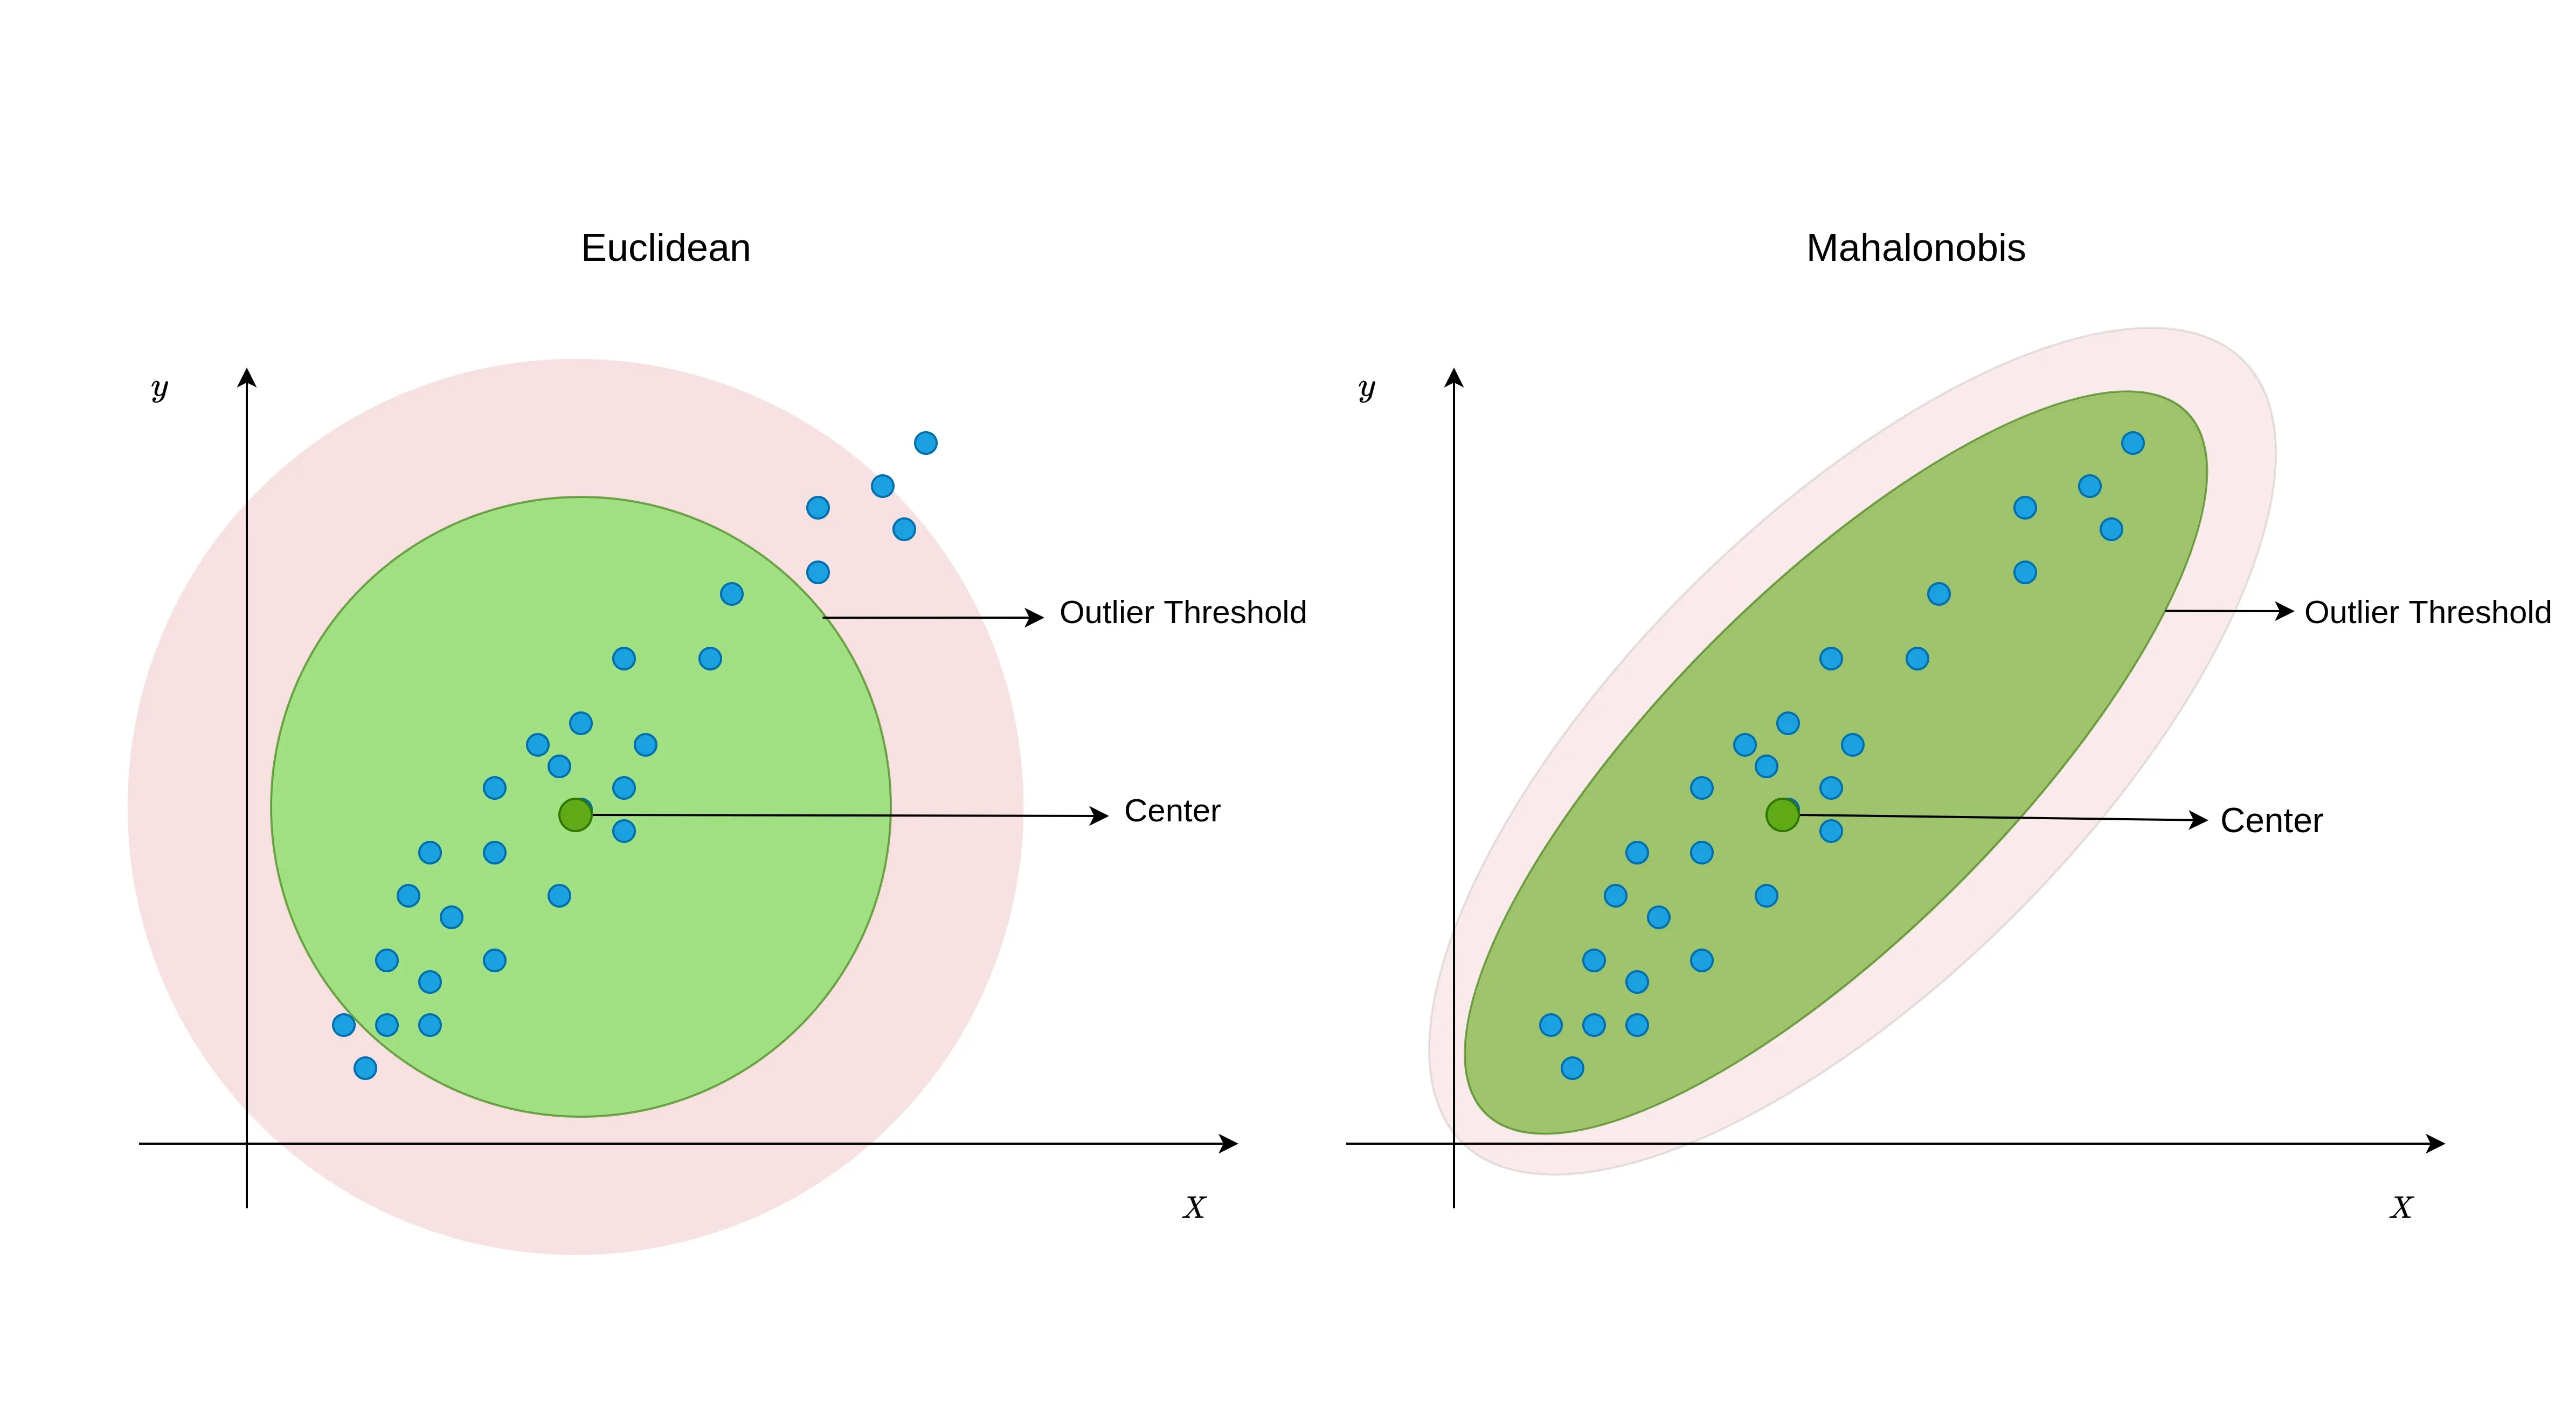
\includegraphics[width=0.9\linewidth]{Pictures/Optimizers/iSAM/Mahalanobis_Distance.png}
    \caption{Euclidean vs.\ Mahalanobis residual contours. \textit{Left:} isotropic (equal) weighting yields circular inlier regions. \textit{Right:} a covariance $\Sigma$ skews and scales the contours into an ellipse whose axes/tilt follow the noise correlations, whitening this with $\Sigma^{-1/2}$ maps this ellipse back to a circle.\textsuperscript{\cite{mahalanobis_distance_explained}}}
    \label{fig:mahalanobis-distance}
\end{figure}
\noindent
Mahalanobis distance is just ``error measured in the units of its noise'' (See Figure \ref{fig:mahalanobis-distance}). If a residual has high variance, we shouldn't punish it as much, if two components are correlated, we shouldn't treat them as independent. That's what the covariance does. In the left plot (Euclidean), all directions are weighted equally so the inlier region is a circle. In the right plot (Mahalanobis), directions with low uncertainty are tighter and correlated axes tilt the ellipse. In our SLAM cost, each residual (process or measurement) is evaluated with its own covariance. Small reliable noises count more, whilst large noisy ones count less. When two parts of a measurement drift together, their error isn't along x or y alone, it's along some tilted direction. Mahalanobis tilts the ``penalty shape'' to match that direction. We are punished less along noisy directions and more where the sensor is precise.
\\ \\
Equation \eqref{eq:optimizer-iSAM-delta-theta-star-mahalanobis-form} is a sum of Mahalanobis residuals (process terms use $\Lambda_i$, measurement terms use $\Gamma_k$). To turn that into one clean least squares system, we ``whiten'' each residual so its noise is unit, for scalars divide by the standard deviation, for vectors apply the covariance's square root inverse to the residual and its Jacobians $\Sigma^{-1}$. After whitening, all errors are ordinary Euclidean ones, so we drop the covariance symbols, stack the Jacobians into one big sparse matrix $A$, stack the prediction errors into $b$, and solve the standard least squares problem \eqref{eq:optimizer-iSAM-delta-theta-star}.
\begin{equation}
    \Delta\theta^\star = \arg\min_{\Delta\theta}\; \|A\Delta\theta - b\|^2
    \label{eq:optimizer-iSAM-delta-theta-star}
\end{equation}
Here, $\theta$ stacks all unknowns (robot poses $x$ and landmarks $l$), $A$ is the single large, sparse (whitened) measurement Jacobian formed by stacking the block Jacobians $F, G, H,$ and $J$ from the linearized motion and measurement models, and $b$ is the stacked prediction error vector that collects the current odometry errors $a$ and measurement errors $c$ with a consistent sign convention. Intuitively, $A$ describes how residuals change for small state perturbations, $b$ encodes the present mismatch between predictions and measurements, and solving equation (\ref{eq:optimizer-iSAM-delta-theta-star}) yields the best local correction $\Delta\theta^\star$ used to update the estimate.
\\ \\
In the linearized setting, the optimal increment $\Delta\theta^\star$ is found by setting the gradient of the least squares objective to zero. This yields the normal equations according to iSAM paper \cite{iSAM_paper}:
$$
    A^{T}A\Delta\theta = A^{T}b
$$
Solving this system is typically performed using a numerically stable square root method (QR/Cholesky) rather than forming an explicit inverse. This gives the optimal correction $\Delta\theta^\star$. The state estimate is then updated as follows:
$$
    \theta \leftarrow \theta + \Delta\theta^\star
$$



\subsubsection{Incremental QR for fast updates (iSAM)}
We solve the linearized SLAM subproblem by least squares. Solving the normal equations $(A^\top A)\Delta\theta = A^\top b$ with Cholesky can be fast but very unstable and ill conditioned as the problem grows (it squares the condition number and increases fill in). iSAM avoids this by working directly with the whitened Jacobian $A$ using QR factorization, and by updating that factorization incrementally when new factors arrive.
\\ \\
Batch square root form (QR on the Jacobian) can be shown in iSAM paper \cite{iSAM_paper} to be of form:

$$
    A \;=\; Q
    \begin{bmatrix}
    R\\[2pt]
    0
    \end{bmatrix},
    \qquad Q^\top Q = I,
    \qquad R \text{: upper triangular}
$$
$$
    \begin{bmatrix}
    d\\ e
    \end{bmatrix}
    \;=\;
    Q^\top b
$$
$$
    \|A\Delta\theta - b\|^2
    \;=\;
    \|R\Delta\theta - d\|^2 + \|e\|^2
$$

\noindent
The iSAM paper \cite{iSAM_paper} shows that after QR we have:
$$
    A\Delta\theta - b \;=\;
    \begin{bmatrix} R \\ 0 \end{bmatrix}\Delta\theta -
    \begin{bmatrix} d \\ e \end{bmatrix},
    \quad\Rightarrow\quad
    \|A\Delta\theta - b\|^2 = \|R\Delta\theta - d\|^2 + \|e\|^2.
$$
\noindent
Put simply, once we do QR, the error splits into two parts. To make the total error as small as possible, we make the first part zero by solving:
\begin{equation}
    R\Delta\theta^\star = d
    \label{eq:optimizer-iSAM-fast-solution}
\end{equation}

\noindent
leaving $\|e\|^2$ as the (minimal) residual norm. If $R$ has full rank, this linearized system has one singular unique solution $\Delta\theta^\star$.
\\ \\
In iSAM the matrix $R$ is upper triangular, so we solve equation (\ref{eq:optimizer-iSAM-fast-solution}) by back substitution (no matrix inverse). This gives a fast, numerically stable way to compute the correction and update the state $\theta \leftarrow \theta + \Delta\theta^\star$ without heavy compute.



\subsubsection{What is R? The square root information matrix}
At the end of QR, the triangular factor $R$ satisfies the following form:
$$
R^\top R \;=\; A^\top A .
$$
This means $A^\top A$ (the information matrix obtained by linearization) is represented by the ``square root'' $R$. Working with $R$ keeps all the curvature of the problem but in a form that is easier to use and numerically safer because $R$ is upper triangular, so computations reduce to cheap substitution methods instead of expensive matrix inverses. Uncertainty can also be extracted directly from $R$. The state covariance is given by:

$$
\Sigma \;=\; (A^\top A)^{-1} \;=\; (R^\top R)^{-1},
$$
We never build a dense inverse. When we need entries of the uncertainty $\Sigma$, we solve small triangular systems with $R^\top$ and $R$ and read only the pose and pose to landmark blocks we care about. Since $R$ is sparse and triangular, this is fast and stable, and we avoid forming $A^\top A$. (See  \ref{sssec:iSAM-data-association} \nameref{sssec:iSAM-data-association})



\subsubsection{Matrix Factorization for building QR (Givens rotations)}
We use \emph{Givens rotations} to build an upper triangular factor $R$ from the (whitened) Jacobian $A$ by zeroing entries below the diagonal, one at a time. This yields a QR factorization without forming $A^\top A$ and without explicitly storing $Q$.
\\ \\
A Givens rotation is a $2\times 2$ orthogonal transform applied to two rows (or two columns) to annihilate one chosen entry. Givens rotation matrix is defined as:
\begin{equation}
    G(\varphi) =
    \begin{bmatrix}
        \cos\varphi & \sin\varphi \\
        -\sin\varphi & \cos\varphi
    \end{bmatrix}
    \label{eq:optimizer-iSAM-givens-rotation}
\end{equation}
Start at the leftmost non zero column of the $A$ matrix and sweep to the right, one column at a time. In each column, pick two rows, \textit{``k''} (the current pivot row) and \textit{``i''} (a row below it), and apply the small ``rotate and combine'' equation (\ref{eq:optimizer-iSAM-givens-rotation}) so the entry under the diagonal in that column becomes zero. Only those two rows are mixed, the new row \textit{``k''} becomes a bit of the old row \textit{``k''} plus a bit of row \textit{``i''}, and the new row \textit{``i''} becomes a bit of the old row \textit{``i''} minus a bit of row \textit{``k''}. Repeat down the column until all subdiagonal entries are gone, then move to the next column on the right. (see Figure \ref{fig:givens-rotation} down bellow for a visual of one Givens step)
\\ \\
As we sweep the columns of $A$, the matrix is transformed into an upper triangular form, this is $R$ and we never need to build the full $Q$. Apply the same row rotations to $b$ as you eliminate entries so the right hand side stays consistent. After the initial factorization of $A$ matrix, new measurements don't require rebuilding $A$. We will illustrate later that we can just append the new (whitened) rows under the current $R$ and apply a short sequence of the same row rotations to re triangularize $R$ matrix again. In other words, updates operate directly on $R$ (and $b$), we bypass $A$ entirely for incremental steps.
\begin{figure}[H]
    \centering
    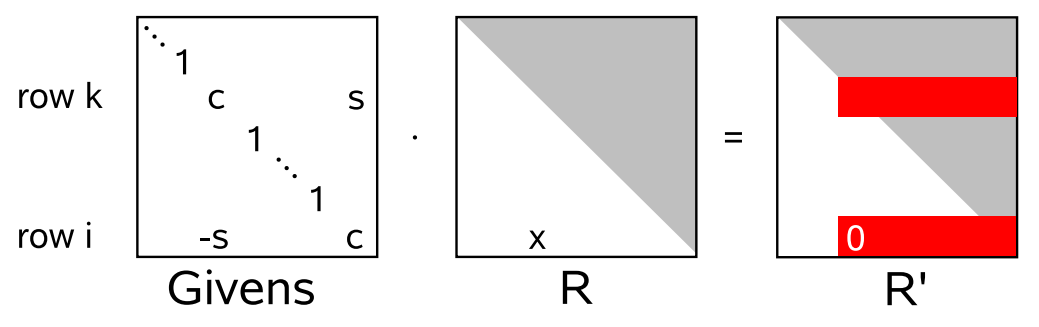
\includegraphics[width=0.9\linewidth]{Pictures/Optimizers/iSAM/Givens_Rotations.png}
    \caption{One Givens step in QR. The entry marked ``x'' is eliminated by rotating two rows, only the entries shown in red are modified, and the exact pattern depends on sparsity. Repeating this column wise (left to right) turns the matrix into an upper triangular $R$. Apply the same rotation to the $b$ vector to keep the least squares system consistent.\textsuperscript{\cite{iSAM_paper}}}
    \label{fig:givens-rotation}
\end{figure}
\noindent
In order to make $R$ upper triangular, we need to get perfect $\varphi$ value to zero a single sub diagonal entry in preliminary matrix, either be it $A$ matrix on batch step or $R$ matrix on iterative steps. we choose a rotation angle $\varphi$ from the two numbers we want to combine in the current column, the pivot $x=a_{kk}$ and the subdiagonal $y=a_{ik}$.
$$
    \begin{aligned}
        r=\sqrt{x^2+y^2}=\sqrt{a_{kk}^2+a_{ik}^2} \\
        c=\cos\varphi=\frac{x}{r}=\frac{a_{kk}}{r} \\
        s=\sin\varphi=\frac{y}{r}=\frac{a_{ik}}{r} 
    \end{aligned}
$$
Solving for $\varphi$ gives us the following answer, where $\alpha = x = a_{kk}$ and $\beta = y = a_{ik}$:
\begin{equation}
    (\cos\varphi,\ \sin\varphi)=
    \begin{cases}
    (1,\,0), & \text{if }\beta=0,\\[6pt]
    \left(-\dfrac{\alpha}{\beta}\,\dfrac{1}{\sqrt{1+(\alpha/\beta)^2}},\ \dfrac{1}{\sqrt{1+(\alpha/\beta)^2}}\right), & \text{if }|\beta|>|\alpha|,\\[10pt]
    \left(\dfrac{1}{\sqrt{1+(\beta/\alpha)^2}},\ -\dfrac{\beta}{\alpha}\,\dfrac{1}{\sqrt{1+(\beta/\alpha)^2}}\right), & \text{otherwise.}
    \end{cases}
    \qquad\text{with }\ \alpha:=a_{kk},\ \beta:=a_{ik}.
    \label{eq:optimizer-iSAM-givens-rotation-find-phi}
\end{equation}
These coefficients in equation \eqref{eq:optimizer-iSAM-givens-rotation-find-phi} give the same rotation as \eqref{eq:optimizer-iSAM-givens-rotation}. They guarantee the $(i,k)$ entry in the working matrix becomes zero, and they do it without changing lengths first for the two number pair $[x,\,y]^\top$ we rotate, and, when embedded, for the affected parts of the two rows (and the matching entries of $b$). In practice, embed $G_{(i,k)}(\varphi)$ so it acts only on rows $k$ and $i$, and apply the same rotation to $b$ to keep the least squares system consistent.



\subsubsection{Incremental Updating}
\begin{figure}[H]
    \centering
    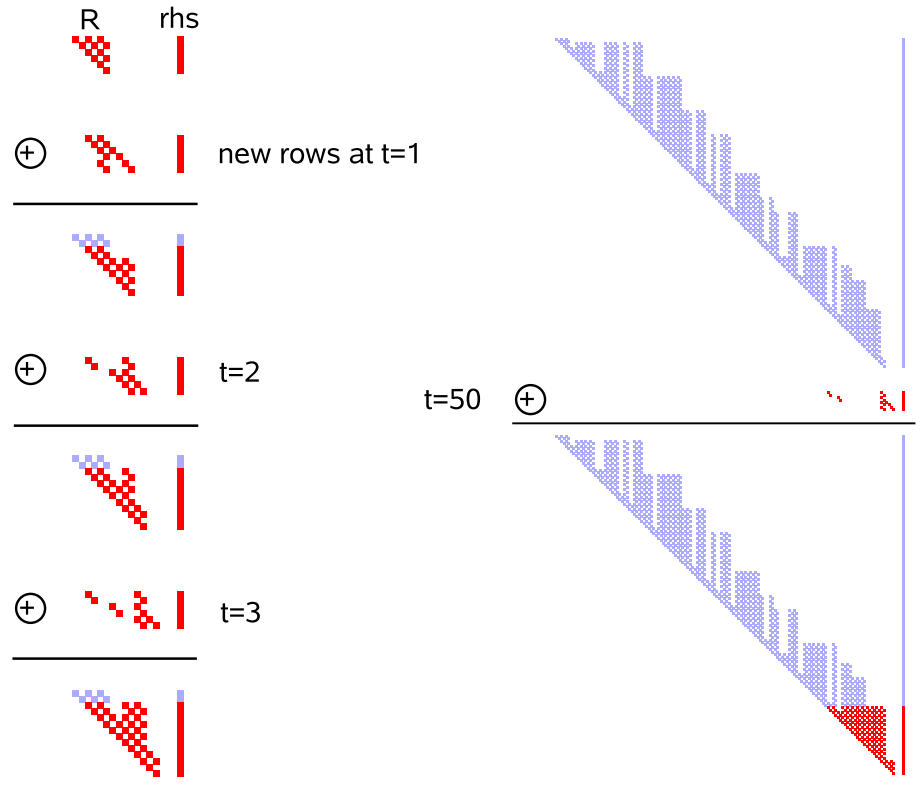
\includegraphics[width=0.5\linewidth]{Pictures/Optimizers/iSAM/R_Matrix_Update_Step.png}
    \caption{Incremental update of the factored system. A new whitened row $w^\top$ and RHS (Right Hand Side) entry $\gamma$ are appended beneath the current $R$ and $d$. A short sequence of Givens rotations restores the upper triangular form, yielding updated $R'$ and $d'$. Unchanged entries are shown in light color, only a small stencil is touched each step, so update cost stays bounded.\textsuperscript{\cite{iSAM_paper}}}
    \label{fig:R-matrix-update-step}
\end{figure}
\noindent
After the initial QR factorization, we maintain the solution in ``square root'' form, an upper triangular matrix $R$ and a transformed right hand side $d$. Here, $R$ is the triangular factor that satisfies $R^\top R = A^\top A$ (the Gauss Newton information), and $d$ is the top part of $Q^\top b$. When a new measurement arrives, we first whiten it (divide by its standard deviation or apply the square root information of its covariance) so it has unit variance. The whitened measurement contributes a new row $w^\top$ to the Jacobian and a new scalar $\gamma$ to the RHS (Right Hand Side). Notice that we do NOT rebuild $A$. Instead, we append $w^\top$ under the current $R$, and $\gamma$ under the current $d$, which produces a system that is ``almost'' triangular but has one non triangular row at the bottom.
$$
    R' = \begin{bmatrix} R\\ w^\top \end{bmatrix},\qquad
    d' = \begin{bmatrix} d\\ \gamma \end{bmatrix}
$$
Next, we re-triangularize locally with Givens rotations \eqref{eq:optimizer-iSAM-givens-rotation}. We only touch the columns where the new whitened Jacobian row $w^\top$ has nonzeros (i.e, the variables that this new factor actually connects to, such as a pose $x_i$ or a landmark $l_j$). Starting from the leftmost such column, each rotation mixes the current pivot row with the new bottom row to kill one sub diagonal entry. We repeat until the entire bottom row is zero and the matrix is upper triangular again. The equation would look something like this:
$$
    \begin{bmatrix} R\\ w^\top \end{bmatrix}
    \ \xrightarrow{\ \text{Givens rotation on affected columns}\ }\ 
    \begin{bmatrix} R'\\ 0 \end{bmatrix}
$$
While we rotate the matrix, we apply the same rotations to the right hand side so that the least squares system stays consistent. Here $d$ is the transformed RHS (Right Hand Side) before the update and $\gamma$ is the new whitened RHS entry that pairs with $w^\top$. After the rotations, the top block becomes the updated RHS $d'$ used for solving, and the final bottom entry becomes a small leftover error $e_{\text{new}}$ that adds to the total residual. 
$$
    \begin{bmatrix} d\\ \gamma \end{bmatrix}
    \ \xrightarrow{\ \text{same rotations}\ }\ 
    \begin{bmatrix} d'\\ e_{\text{new}} \end{bmatrix}
$$
Intuitively, the new row $w^\top$ is ``folded up'' into the triangular structure by a short chain of 2x2 rotations that only touch the connected variables, everything else is left alone. We then get the correction by a fast back substitution on the updated matrix $R'$ and vector $d'$:
$$
    R'\Delta\theta^\star = d'
$$



\subsubsection{Loop Closure}
\begin{figure}[H]
    \centering
    % ---------- Left column ----------
    \begin{minipage}[t]{0.48\linewidth}
        \vspace{0pt}
        % Top-left (image 1)
        \begin{subfigure}[t]{\linewidth}
            \centering
            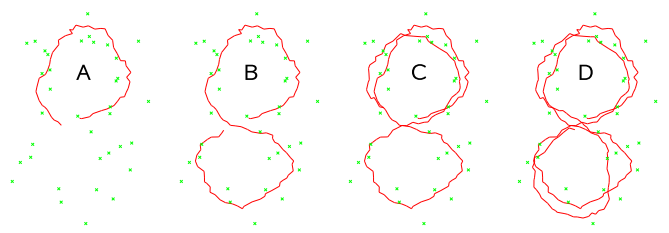
\includegraphics[width=\linewidth,height=0.47\textheight,keepaspectratio]{Pictures/Optimizers/iSAM/Variable_Reordering1.png}
            \caption{Simulated double 8 loop at key loop closure moments.\textsuperscript{\cite{iSAM_paper}}}\label{fig:l-top}
        \end{subfigure}\vspace{4pt}

        % Bottom-left row: (2) and (3) side-by-side
        \begin{subfigure}[t]{0.49\linewidth}
            \centering
            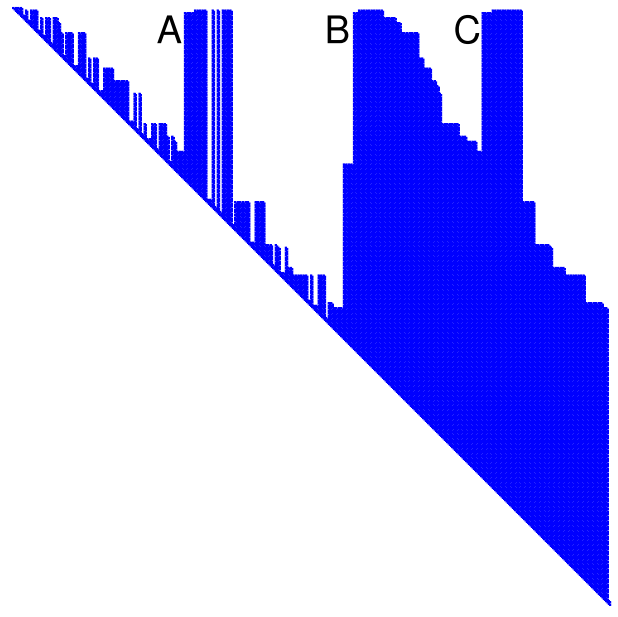
\includegraphics[width=\linewidth,height=0.20\textheight,keepaspectratio]{Pictures/Optimizers/iSAM/Variable_Reordering2.png}
            \caption{Upper triangular factor $R$ after several closures shows fill-in.\textsuperscript{\cite{iSAM_paper}}}\label{fig:l-bot-left}
        \end{subfigure}\hfill
        \begin{subfigure}[t]{0.49\linewidth}
            \centering
            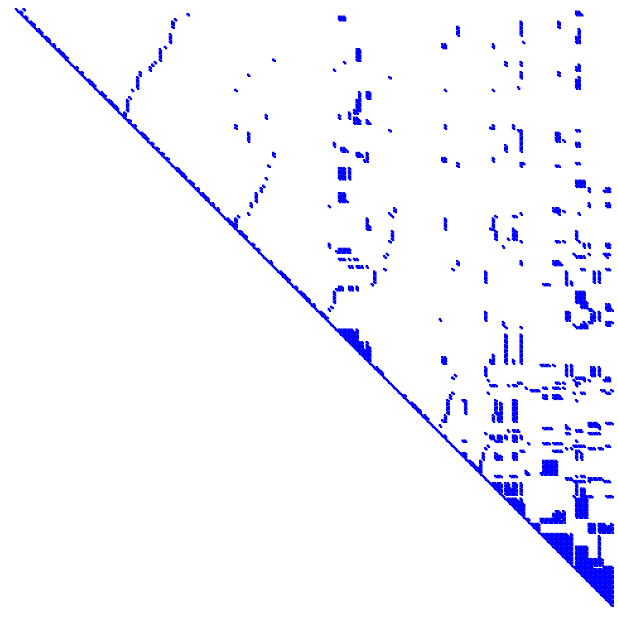
\includegraphics[width=\linewidth,height=0.20\textheight,keepaspectratio]{Pictures/Optimizers/iSAM/Variable_Reordering3.png}
            \caption{The same $R$ after variable reordering (COLAMD) becomes sparser again.\textsuperscript{\cite{iSAM_paper}}}\label{fig:l-bot-right}
        \end{subfigure}
    \end{minipage}\hfill
    % ---------- Right column ----------
    \begin{minipage}[t]{0.49\linewidth}
        \vspace{0pt}
        \begin{subfigure}[t]{\linewidth}
            \centering
            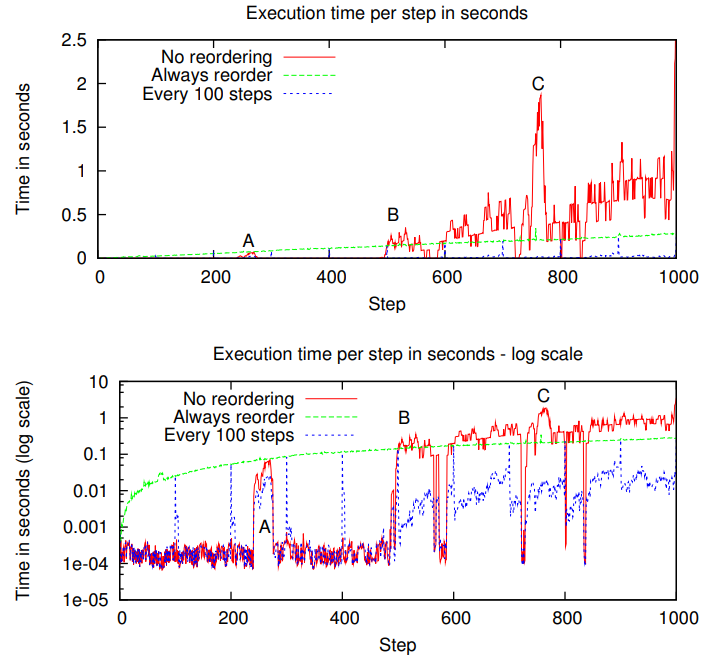
\includegraphics[width=\linewidth,height=0.98\textheight,keepaspectratio]{Pictures/Optimizers/iSAM/Variable_Reordering4.png}
            \caption{Per step execution time for three strategies. A: no reordering, B: reorder every step, C: reorder every 100 steps, shown in linear (top) and log (bottom) scale. Periodic reordering (C) limits spikes and keeps runtime predictable between loop closures.\textsuperscript{\cite{iSAM_paper}}}\label{fig:r-full}
        \end{subfigure}
    \end{minipage}

    \caption{Effect of loop closures and variable reordering (iSAM).\textsuperscript{\cite{iSAM_paper}}}
    \label{fig:variable-reordering}
\end{figure}
\noindent
Loop closures tie together far-apart parts of the trajectory (and landmarks), which makes previously separate columns interact. In QR terms this creates fill-in, R gets extra non zeros, so updates, back substitution, and selected covariance queries get slower and memory grows. We fix this by variable reordering. What we do is pick a new elimination order that preserves sparsity. In practice we run a heuristic like \gls{COLAMD} (Column Approximate Minimum Degree) (often the block version for pose/landmark blocks) on the Jacobian's sparsity matrix $A$, then do batch factorization on the whole $A$ matrix using rotations \eqref{eq:optimizer-iSAM-givens-rotation} with that order \cite{iSAM_paper}. Reordering costs time because we rebuild the factor with a new permutation, but it pays back by making the next many updates cheap again.
\\ \\
Because reordering is expensive, we don't do it every step. Instead we do periodic reorder every N steps (eks, 50 - 200) so cost stays predictable. In marine \gls{AUV} runs this keeps compute bounded. Between reorders incremental updates are fast and local. After a loop closure, we accept one spike (reorder + refactor), then return to low latency. Practical tips when doing this step is to keep poses as blocks (block \gls{COLAMD}) to reduce fill-in, align reordering with planned relinearization passes, and monitor simple stats (nonzeros in R, update time) to decide when N is too small (wasting time reordering) or too large (letting fill in snowball).  



\subsubsection{Re-Linearization}
Re-linearization keeps the local model honest. All the QR/update tricks we have gone through now assume the system is locally linear around the current estimate, but with angles, 3D motion, and nonlinear sensors that linearization drifts as the robot moves. If we never refresh it, increments stop being small, the optimizer biases the map, and loop closures can break the solution. The fix is to re-linearize, recompute Jacobians at the current state for the factors that matter. Doing this for every factor at every step is too expensive, so in practice we always linearize new factors (fresh odometry and measurements) and refresh older ones only when needed.
\\ \\
In iSAM the practical schedule is to perform incremental updates between maintenance cycles, then do a full re-linearization at a fixed interval N. Between cycles we do not re-linearize old factors, we only whiten and insert the new ones and update $R$ incrementally. At the cycle boundary when we hit N steps, we re-linearize the entire problem at the current estimate (conceptually rebuild the full Jacobian $A$), run a variable reordering to restore sparsity using \gls{COLAMD}, and refactor using equation \eqref{eq:optimizer-iSAM-givens-rotation} to get a fresh triangular $R$. Thats why we usually bunch variable reordering with batch linearization in the same N step. 
\\ \\
We must choose $N$ carefully, by balancing freshness vs compute. If N is too large, the linearization point drifts far from reality, Jacobians no longer match the true geometry, corrections become biased, loop closures pull hard, and the map can warp (a classic ``stale linearization'' issue). If N is too small, we keep stopping to relinearize and refactor, burning CPU and power and hurting real-time throughput.



\subsubsection{Data Association from R}\label{sssec:iSAM-data-association}
For data association we often use a Mahalanobis based approach instead of plain nearest neighbour Approach. Nearest neighbour measures raw Euclidean distance and ignores sensor noise and correlations. Mahalanobis measures the innovation in the units of its uncertainty, so noisy directions count less, precise directions count more, and correlated components are handled correctly (See Figure \ref{fig:mahalanobis-distance}). For a candidate match between current pose $x_i$ and landmark $l_j$, form the innovation $\nu_k$ and score:
$$
    d_k^2=\nu_k^\top\,\Xi_k^{-1}\,\nu_k,\qquad
    \Xi_k=J_k\,\Sigma\,J_k^\top+\Gamma_k
$$
\noindent
where $J_k=[\,H^{x_i}\ \ H^{l_j}\,]$ is the linearized measurement Jacobian, $\Gamma_k$ is the sensor noise, and $\Sigma$ is the state covariance. 
\\ \\
This type of data association often uses gating with a chi-square test. The test keeps matches that are within $d_k^2\le \chi^2_{m,\alpha}$ (right dimension $m$, chosen confidence $\alpha$). From the survivors, we pick the ``minimum cost'' one (or solve a global assignment using $d_{ij}^2$ as the cost matrix if several features compete). One thing to note about this approach is that we don't need the full dense $\Sigma=(R^\top R)^{-1}$ to do our data association, we only require local covariances touched by the measurement. These types of covariances can be pull directly from the square root information matrix $R$. Here we can get pose, and pose to landmark terms are available live. Landmark terms on the other hand are either a approximate fast conservative estimate or computed exactly on demand. This keeps the association real-time for the most part.
Here are the partitioned forms.
Full state covariance (poses vs. landmarks):
$$
    \Sigma \;=\;
    \begin{bmatrix}
    \Sigma_{xx} & \Sigma_{xL}\\[4pt]
    \Sigma_{Lx} & \Sigma_{LL}
    \end{bmatrix}
$$
\noindent
where $\Sigma_{xx}$ is pose to pose, $\Sigma_{LL}$ is landmark to landmark, and $\Sigma_{xL}=\Sigma_{Lx}^\top$ is pose to landmark.
\\ \\
The $2\times2$ submatrix needed for a single candidate $(x_i,l_j)$:
$$
\Sigma_{\{x_i,l_j\}} \;=\;
\begin{bmatrix}
\Sigma_{x_i x_i} & \Sigma_{x_i l_j}\\[4pt]
\Sigma_{l_j x_i} & \Sigma_{l_j l_j}
\end{bmatrix}
$$
\noindent
\textbf{Fast marginals from the square root factor (online/live)} 
\\ \noindent
In iSAM paper \cite{iSAM_paper}, they propose keeping the current pose last in the ordering. Then the covariances needed for association, the pose variance $\Sigma_{x_i x_i}$ and the pose to landmark cross terms $\Sigma_{x_i l_j}$ come straight from the square root factor $R$ with two small triangular solves:
$$
    R^\top Y = B,\qquad R X = Y
$$
where $B=\begin{bmatrix}0\\ I_{d_x}\end{bmatrix}$ simply selects the last pose block of size $d_x$. Because $R$ is upper triangular and $B$ is zero above the last block, the forward solve gives:
$$
Y=\big[\,0,\ldots,0,\ R_{ii}^{-1}\,\big]^\top
$$
This $Y$ preliminary matrix is the clue, where only $d_x$ back substitutions are needed to get full $X$ vector. Reading the result $X$ yields, in one pass:
$$
\Sigma_{x_i x_i} \;\; \text{(bottom–right block of } \Sigma)\qquad
\Sigma_{l_j x_i}=\Sigma_{x_i l_j}^\top \;\; \text{for connected } l_j
$$
Intuitively we ``solve up'' then ``solve down'' on $R$ for the last pose, and we get exactly the columns of $\Sigma=(R^\top R)^{-1}$ that matter for gating in data association. This can be done every step without forming any dense inverses, only using $R$ square root information matrix iteratively. (See Figure \ref{fig:mahalanobis-distance})
\begin{figure}[H]
  \centering
  \begin{subfigure}[t]{0.49\linewidth}
    \centering
    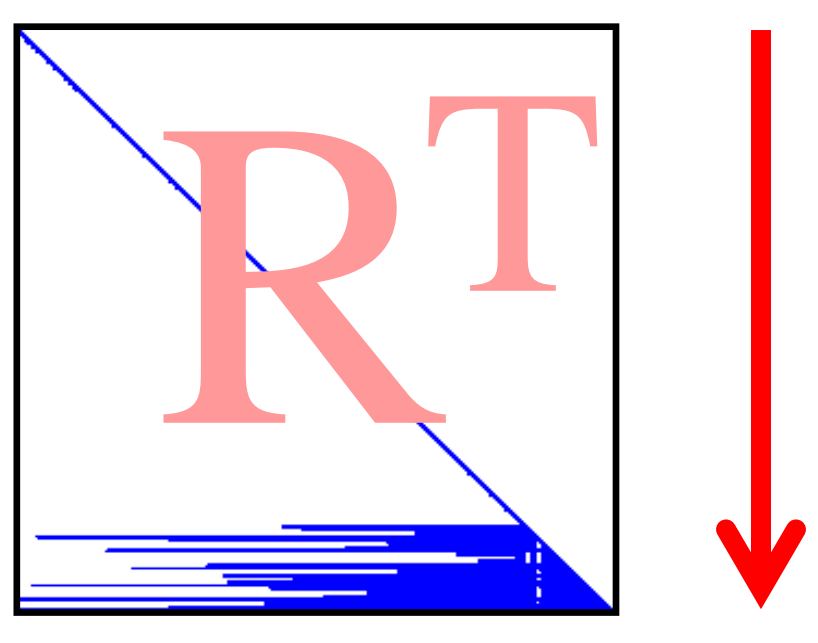
\includegraphics[width=\linewidth]{Pictures/Optimizers/iSAM/Substitution_Forward.png}
    \caption{$R^\top Y = B$ (forward substitution). Sweep ``down'' the matrix to form $Y$ from a selector $B$ that picks the last pose block.}
    \label{fig:left}
  \end{subfigure}\hfill
  \begin{subfigure}[t]{0.49\linewidth}
    \centering
    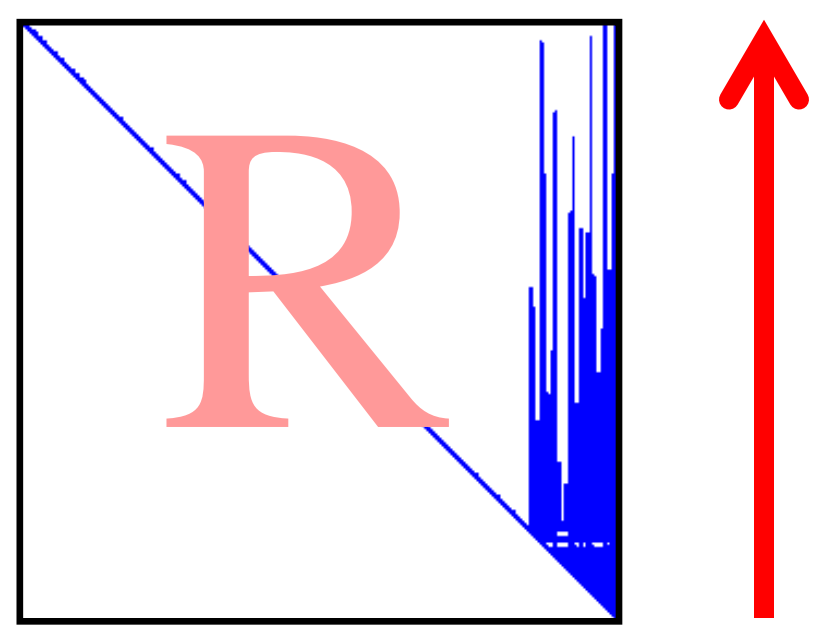
\includegraphics[width=\linewidth]{Pictures/Optimizers/iSAM/Substitution_Downwards.png}
    \caption{$R X = Y$ (back substitution). Sweep ``up'' the matrix to obtain the desired columns $X=\Sigma_{:\,,x_i}$ (pose and pose to landmark).}
    \label{fig:right}
  \end{subfigure}
  \caption{We grab the needed covariances in two quick steps: first solve ``down'' with $R^\top$, then solve ``up'' with $R$. We only touch entries near the last pose block, so each update stays fast and cheap.\textsuperscript{\cite{iSAM_paper}}}
  \label{fig:substitution-foward-backwards}
\end{figure}
\noindent
\textbf{Conservative landmark covariances (online/live)} 
\\ \noindent
Exact landmark landmark blocks $\Sigma_{jj}$ (or old pose to landmark $\Sigma_{(i-n)j}$) are expensive to extract at every step. Therefore in iSAM paper \cite{iSAM_paper} they propose using a safe, conservative bound built from the current pose covariance and the measurement noise via the linearized back projection:
$$
    \tilde\Sigma_{jj}
    \;=\;
    \bar J\,
    \begin{bmatrix}
    \Sigma_{ii} & 0\\[2pt]
    0 & \Gamma
    \end{bmatrix}
    \bar J^\top
$$
where $\bar J$ is the Jacobian of the local inverse measurement model, $\Sigma_{ii}$ is the current pose covariance, and $\Gamma$ is the measurement noise. This upper bounds landmark uncertainty (never over confident), is fast, and works well for online Mahalanobis gating. As more measurements of a landmark arrive, this bound typically tightens.
\\ \\
An important caveat to mention is that we usually don't know the true $\Gamma$ (measurement noise) exactly. The iSAM recipe is to choose $\Gamma$ conservatively so we don't get over confident. That keeps things safe but can make the gate too tight, causing the data association to reject more matches than it should. Later, we will discuss a more confident way to approximate $\Gamma$ from measurement characteristics without being overly confident (eks: range/resolution for sonar and landmark confidence) so the gate is realistic without being risky.
\\ \\
\textbf{Exact landmark covariances (on demand)} 
\\ \noindent
When we need accuracy (eks: on risky loop closure, conflicting hypotheses), Data Association can recover exact $\Sigma_{jj}$ and $\Sigma_{(i-n)j}$ without forming the full dense inverse information matrix $\Sigma=(A^{T}A)^{-1}=(R^{T}R)^{-1}$. Because the covariance is the inverse of the information matrix:
$$
    \Sigma=(R^\top R)^{-1}, \qquad R^\top R\,\Sigma = I
$$
We can get the needed entries without forming the full inverse by solving for two triangular matrixes:
$$
R^\top Y = I, \qquad R \Sigma = Y
$$
We only follow the ``nonzeros'' of $R$ when solving. That means we don't touch the whole matrix, just the parts that matter. iSAM walks backwards along those non zero links and gives us exactly the covariance numbers $\sigma_{ij}$ Data Association ask for. If $R$ is mostly banded, this is near linear time. We should only use this exact method when we really need it (eks: a few $\Sigma_{jj}$ blocks to check on a loop closure). It's slower than the conservative shortcut, but still much faster than inverting the whole matrix.
\\ \\
\textbf{Alternative way to finding $\Gamma$} 
\\ \noindent
There's another angle. Instead of being very conservative with our $\Gamma$ measurement noise. Uncertainty used in Data Association should reflect the sensor, for example a sonar for scanning the sea floor. With sonar we can make the measurement noise grow with range and use the transducer's resolution to set per axis variances $N(0, \Sigma_{sonar})$. The landmark detection can also contribute its own uncertainty $N(0, \Sigma_{landmark})$. In practice we could combine ``sensor noise'' and ``landmark estimate noise'' to get the prediction uncertainty for the residual we score. In that case we can say:
$$
    \Gamma = Var(h(x, l)) = \Sigma_{sonar} + \Sigma_{landmark}
$$
This can be more informative than a one size fits all setting. However we must be very careful with this approach, if we make these noises too optimistic, the gate in Data Association gets too tight, associations become brittle, and the system can go unstable. Never the less this is a lot better approach for building more accurate maps and estimating robots track.



\subsubsection{Algorithm}
At each time step we absorb new information, linearize around the current estimate, solve a small least squares, and update. Periodically we refresh linearization and variable order. Concretely:
\begin{enumerate}
    \item \textbf{Add factors (whiten first):} take the new odometry/measurements and add them to the graph. ``Whiten”'' them so every residual has unit noise (as described before \eqref{eq:optimizer-iSAM-delta-theta-star}).

    \item \textbf{Linearize at the current guess \(\theta\):} turn the nonlinear motion/measurement models into local linear ones using the Jacobians in
    \eqref{eq:optimizer-iSAM-linearized-odometry} and \eqref{eq:optimizer-iSAM-linearized-measurement}. This gives the summed Mahalanobis cost \eqref{eq:optimizer-iSAM-delta-theta-star-mahalanobis-form}, which after whitening becomes one least squares problem \eqref{eq:optimizer-iSAM-delta-theta-star}.

    \item \textbf{Keep a triangular system up to date (QR):} append the new (whitened) rows and apply a few Givens rotations \eqref{eq:optimizer-iSAM-givens-rotation} so the matrix stays upper triangular $R$. Update the right hand side $b$ vector the same way (see ``Incremental Updating'').

    \item \textbf{Solve for the small change:} because $R$ is triangular, solve
    \eqref{eq:optimizer-iSAM-fast-solution} by back substitution (fast) to get the correction .

    \item \textbf{Update the estimate:} replace the old state with the improved one,
    $\theta \leftarrow \theta + \Delta\theta^\star$.

    \item \textbf{Every \(N\) steps (maintenance):} refresh accuracy by re-linearizing all factors at the new $\theta$, reorder variables (eks: COLAMD algorithm) to keep things sparse, and refactor with Givens \eqref{eq:optimizer-iSAM-givens-rotation} to get a clean $R$.

    \item \textbf{Data Association update:} read the needed covariances from $R$ (pose and pose to landmark live, landmark blocks conservative or exact on demand) and run Mahalanobis gating in Data Association for next matches.
\end{enumerate}



\subsubsection{Limitations}
iSAM is fast between updates but has practical downsides. They come from the ``data structure'', not the underlying SLAM algorithm. iSAM keeps a single, global square root information matrix $R$ (from $A^\top A$) and does periodic maintenance (reordering + re-linearization). This makes updates simple, but couples cost to global structure and variable ordering instead of just local changes.
\begin{itemize}
    \item \textbf{Latency spikes at maintenance:} Periodic global variable reordering and re-linearization trigger stalls (especially after loop closures), since $R$ must be refactored end to end.

    \item \textbf{Fill in growth between reorders:} Incremental QR on a fixed order accumulates fill in in $R$, touching more entries per update and increasing time/memory step by step.

    \item \textbf{All or nothing re-linearization:} iSAM typically refreshes many factors at maintenance even if most variables barely moved, wasting Jacobian recomputations.

    \item \textbf{Global refactor on ordering changes:} Any change to elimination order implies a large refactor of the global $R$, regardless of how small the new information is.

    \item \textbf{Broad marginal queries are costly:} Last pose and nearby cross terms can be pulled quickly from $R$, but wide $\Sigma$ blocks (eks: many landmarks or older poses) require multiple triangular solves and can be costly.

    \item \textbf{Schedule sensitivity:} Choosing ``every $N$ steps'' for reorder/re-linearize is heuristic, too small wastes time, too large lets fill in and linearization error grow, causing jitter and warp in the map.

    \item \textbf{Numerical robustness vs simplicity:} Working with $A$ and $R$ avoids explicit $A^\top A$, but long incremental runs plus fill in can still hurt conditioning and stability if ordering lags.
\end{itemize}
\noindent
These limitations motivated \textbf{iSAM2}, which replaces the single monolithic $R$ that is very static, with a Bayes tree representation that is dynamic and updates only the affected parts. We address iSAM2 and how it mitigates the issues above in the next chapter.

